\clearpage
\section{Versioned chemical audit and controlled-output reconciliation}
The expanded audit inspected 740 valid geometry files, 2675 artifact paths, and 45 CHO/COH-named or graph-identified aliases, including excluded, incomplete and duplicate structures. Twenty-six candidate aliases are retained ML configurations. Identity uses complete molecular graphs: H bonded to carbon identifies CHO, H bonded to oxygen identifies COH, and disconnected CO/H components remain CO+H. Both in-plane minimum images and the nonperiodic vacuum direction are explicit. Cutoffs are scaled by 0.9 and 1.1; ambiguous outcomes require review. No retained target mismatch or ambiguous retained candidate was demonstrated. The six retained COH directories have CHO basenames but observed O--H connectivity. No targets or frozen results are silently overwritten.

\begin{table}[htbp]\centering\begin{tabular}{lrrrr}\toprule Inventory & CHO only & CHO mixtures & All CHO & All COH\\\midrule Retained 87 &2&3&5&6\\ Unique 155 &2&11&13&15\\\bottomrule\end{tabular}\caption{Existing configuration labels, cross-checked with the geometry audit where available. These are configurations, not molecule counts. Single species can mean multiple molecules. Inventory labels are not universal independent validation of every incomplete structure.}\end{table}

The retained CHO mixtures are the interface-Cu, interior-Cu, and uniform CHO 0.056/0.111 entries with CHO;CO;H labels; CHO-only entries are the AuCu- and CuCu-bidentate 0.056 structures. Per-molecule and configuration CSV/JSON tables retain paths, hashes, C--H/O--H distances, bonds, metal contacts, interface distance, intended/relaxed/XAS-used graphs, targets, and inclusion reasons. All available full-cell XAS decks and geometry copies are compared with relaxed coordinates. Element-wise minimum-distance atom assignment detects exact copies and reordered indices, but is not a trajectory-based proof of hydrogen identity exchange in changed geometries. Enlarged local figures display H with a dark border, numbered atoms and explicit bonds; the saved code operates on the frozen audit arrays.

\begin{table}[htbp]\centering\small\begin{tabularx}{\textwidth}{llX}\toprule State & Region & Expanded-search outcome\\\midrule 2CO & Interface & Attempt located; no valid relaxed output or verified spectrum for the pinned input.\\2CO & Terrace & Completed usable record recovered, with intact two-CO connectivity; initial input differs from pinned quartet. Requires lineage reconciliation or regenerated pinned version before this controlled contrast.\\OCCO & Interface & Pinned relaxed geometry and matched Cu spectrum not located; never-run status is not established.\\OCCO & Terrace & Pinned relaxed geometry and matched Cu spectrum not located; never-run status is not established.\\\bottomrule\end{tabularx}\caption{Quartet status derives from recovered artifacts. Equivalent duplicate relaxed geometries count as one outcome. C/O edges are extensions, not prerequisites for the first valid Cu contrast.}\end{table}

Among 102 record attempts, 101 passed geometry/grid/absorber checks and one incompatible grid remains excluded. Seven equal-formula hydrogenation candidates were screened against the same initial metal parent, equal elemental loading, numerical controls and absorber populations, initial in-plane C/O pattern RMS at most 0.75~\AA{}, and relaxed interface-distance mismatch at most 0.5~\AA{}. None passes all checks. Thresholds and each rejection are explicit; equal formula is insufficient. No intended intact-OCCO spectrum is inferred from a changed graph. An intact OCCO-plus-four-CO relaxed geometry is a different loading and has no completed spectrum in the search.

The clean search starts at plain/CONTCAR and plain/2fixed/CONTCAR and also examines all saved XAS geometry copies and raw convolved files. Both clean relaxed structures exist, but no compatible numeric clean spectrum was located. The absence of an AI-ready record alone is not the criterion. Consequently no adsorbate-minus-clean or coupling difference is calculated. Such a difference must retain a shared per-absorber scale and compatible parent, layers, settings, polarization and energy convention; independently min--max normalized absorption cannot be subtracted as a physical contrast. Separately relaxed and frozen-metal controls have different meanings. Prepared clean full-cell decks and quartet relaxation inputs contain no licensed potentials and were not submitted. Exact missing paths and hashes accompany the status CSV.

\section{Nested ML extensions and their limits}
The primary frozen 87-configuration/348-spectrum archive is unchanged. H recall is 14/14 in single-species configurations and 0/8 in mixtures; CO is 21/21 and 5/9. These counts reproduce the supplied cross-check. The exploratory fixed winner is separate. No new fit on these repeatedly examined folds is independent confirmation.

All new recipes use the frozen outer folds and three inner grouped folds. Spectra alone enter predictors; filenames, species/counts, graph/site/coverage/interface descriptors and parent strings define audits, targets or groups only. The surface-layer spectra are cropped to 8976--9027~eV so every predeclared shift of up to 2~eV has native support without extrapolation. The archived full-grid primary is an explicitly different frozen comparator. Existing normalized spectra, CDF and derivatives are included as controls rather than called new. New descriptor windows are fixed at 8976--8985, 8985--8998, 8998--9012 and 9012--9027~eV from edge-relative assumptions, before inspecting test scores; Figure~3's label-conditioned curves do not choose them. Each window yields area, centroid, derivative mean/max/min, peak energy and height. DCT 8/16/24/32 and PCA 8/16 are candidates; PCA/scalers are fitted on training partitions alone. DCT24 retains its historical fixed-candidate meaning.

Nearest neighbors tests cosine/Euclidean and k=1/3/5 inside training, with closest training examples returned for review. Independent Extra Trees and a sequential probability-chain variant each test two compact regularized configurations (32 trees, minimum leaf 2 or 4). Chain training uses group-out-of-fold independent predecessor proxy probabilities; inference proceeds sequentially without true labels. This is explicitly a proxy-chain variant, not an unrestricted co-occurrence generalization claim. Canonical/training-prevalence orders are considered only inside training. Independent per-target XGBoost tests 48/80 rounds, depths 2/3, learning rate 0.05, regularization 5/10, alpha 0.1, minimum child weight 3, row/column fractions 0.8, and training-class weights capped at 10. There is no early stopping against outer folds. Single-class partitions use constant predictors. The saved protocol gives every candidate and missing-positive partition.

Platt calibration uses inner grouped OOF scores only and is unsupported with fewer than five positives or negatives or constant scores. Threshold candidates are 0.15, 0.25, 0.35, 0.45, 0.50, 0.55, 0.65 and 0.75; the global micro-F1 threshold and supported per-label refinements use inner data only. Feature and hyperparameter winners likewise use inner scores. The compact search remains exploratory on repeatedly examined configurations.

\begin{table}[htbp]\centering\small
\caption{Frozen primary and new nested extensions. Aug. denotes training-only synthetic augmentation. New recipes use the common cropped window; these are repeated evaluations of the same configurations.}\label{tab:extensions}
\begin{tabular}{lrrr}\toprule Recipe & Micro F1 & Macro F1 & Exact set\\\midrule
frozen primary & 0.779 & 0.638 & 0.690\\
nearest neighbor & 0.733 & 0.607 & 0.690\\
nearest neighbor + aug. & 0.714 & 0.567 & 0.701\\
independent trees & 0.650 & 0.476 & 0.517\\
independent trees + aug. & 0.674 & 0.502 & 0.552\\
classifier chain & 0.671 & 0.505 & 0.563\\
classifier chain + aug. & 0.663 & 0.476 & 0.552\\
xgboost & 0.614 & 0.440 & 0.425\\
xgboost + aug. & 0.596 & 0.371 & 0.494\\
\bottomrule\end{tabular}\end{table}


None exceeds the primary overall micro F1. Nearest neighbors recovers H 3/8 and CO 6/9 mixtures, with lower overall micro F1; H false positives rise from one to four and CO false positives from zero to two; single-species CO recall falls from 21/21 to 19/21. Per-species precision is reported below rather than treating mixture recall alone as improvement. Paired configuration bootstrap intervals use 500 resamples of fixed OOF predictions; nearest-neighbor micro-F1 change is $-0.046$ (conditional 95\% interval $[-0.139,0.051]$). These intervals omit refitting/selection variation and do not establish superiority. Refit learning curves separately use fractions 0.25/0.5/0.75/1 and seeds 11/23/47 for a predeclared DCT16 tree recipe with threshold 0.5.

Synthetic stress tests are shifts $\pm0.2/0.5/1/2$~eV, extra Gaussian sigma 0.25/0.5/1~eV, and noise 1/2/5\% of native peak intensity. They are scenarios, not measured instrument uncertainty. Positive finite-domain-normalized Gaussian kernels preserve native lifetime treatment. Training-only augmentation supplies one additional combined random $\pm0.5$~eV shift, sigma 0.5~eV Gaussian and 2\% noise copy per training configuration. All copies stay in that configuration's fold. Seed 20261022 and perturbations are frozen in the protocol; stress scores do not select models.

The harder evaluation holds out 56 exact initial-metal coordinate groups across three folds, using a predeclared DCT16 independent-tree recipe with training-only thresholds. Its micro/macro F1 and exact-set accuracy are 0.620/0.470/0.552. These coordinate groups are not verified independent ancestral parents; actual parent transfer cannot be estimated from unverified ancestry. Missing-positive labels are reported per split. No generalization to experimental spectra, new compositions or applied potentials is established.

Review curves use minimum calibrated threshold margin among supported labels, excluding predicted unsupported positives; sparse-label uncertainty remains unresolved and no certified full-set risk is claimed. Predictions expose the identity set, scores, thresholds, unsupported calibration and energy/depth/parent domain flags. A local natural-language agent request calls the shared audited-training API, fits the declared recipe, saves/reloads all 40 fold models, predicts held-out records and saves a sanitized review report. All round trips match exactly. This uses available records; no scheduler or new-spectrum execution is implied. Proposed next actions distinguish scientific controls (clean/coupling, matched CO/H, independent hydrogenated C1/C2 with a locked confirmation set) from disagreement review of existing cases. Proposed calculations have not improved a measured result.

\small\begin{longtable}{llrrrr}
\caption{Per-species extension precision (P), recall (R), F1 and independent configuration support. Aug. is training-only augmentation.}\\
\toprule Recipe & Species & P & R & F1 & Support\\\midrule\endfirsthead
\toprule Recipe & Species & P & R & F1 & Support\\\midrule\endhead
nearest neighbor & CHO & 1.000 & 0.600 & 0.750 & 5\\
nearest neighbor & CO & 0.926 & 0.833 & 0.877 & 30\\
nearest neighbor & CO2 & 0.400 & 0.667 & 0.500 & 3\\
nearest neighbor & COCHO & 0.000 & 0.000 & 0.000 & 1\\
nearest neighbor & COH & 0.429 & 0.500 & 0.462 & 6\\
nearest neighbor & COOH & 0.667 & 0.750 & 0.706 & 8\\
nearest neighbor & H & 0.800 & 0.727 & 0.762 & 22\\
nearest neighbor & O & 0.667 & 0.857 & 0.750 & 7\\
nearest neighbor & OCCOH & 0.500 & 0.500 & 0.500 & 4\\
nearest neighbor & OCHO & 0.800 & 0.500 & 0.615 & 8\\
nearest neighbor & OH & 1.000 & 0.600 & 0.750 & 5\\
nearest neighbor + aug. & CHO & 0.333 & 0.200 & 0.250 & 5\\
nearest neighbor + aug. & CO & 0.960 & 0.800 & 0.873 & 30\\
nearest neighbor + aug. & CO2 & 0.400 & 0.667 & 0.500 & 3\\
nearest neighbor + aug. & COCHO & 0.000 & 0.000 & 0.000 & 1\\
nearest neighbor + aug. & COH & 0.750 & 0.500 & 0.600 & 6\\
nearest neighbor + aug. & COOH & 0.714 & 0.625 & 0.667 & 8\\
nearest neighbor + aug. & H & 1.000 & 0.682 & 0.811 & 22\\
nearest neighbor + aug. & O & 0.667 & 0.857 & 0.750 & 7\\
nearest neighbor + aug. & OCCOH & 0.667 & 0.500 & 0.571 & 4\\
nearest neighbor + aug. & OCHO & 0.444 & 0.500 & 0.471 & 8\\
nearest neighbor + aug. & OH & 1.000 & 0.600 & 0.750 & 5\\
independent trees & CHO & 1.000 & 0.200 & 0.333 & 5\\
independent trees & CO & 1.000 & 0.833 & 0.909 & 30\\
independent trees & CO2 & 0.500 & 0.667 & 0.571 & 3\\
independent trees & COCHO & 0.000 & 0.000 & 0.000 & 1\\
independent trees & COH & 1.000 & 0.333 & 0.500 & 6\\
independent trees & COOH & 0.286 & 0.250 & 0.267 & 8\\
independent trees & H & 0.923 & 0.545 & 0.686 & 22\\
independent trees & O & 1.000 & 0.143 & 0.250 & 7\\
independent trees & OCCOH & 0.667 & 0.500 & 0.571 & 4\\
independent trees & OCHO & 1.000 & 0.250 & 0.400 & 8\\
independent trees & OH & 1.000 & 0.600 & 0.750 & 5\\
independent trees + aug. & CHO & 0.000 & 0.000 & 0.000 & 5\\
independent trees + aug. & CO & 0.926 & 0.833 & 0.877 & 30\\
independent trees + aug. & CO2 & 0.286 & 0.667 & 0.400 & 3\\
independent trees + aug. & COCHO & 0.000 & 0.000 & 0.000 & 1\\
independent trees + aug. & COH & 1.000 & 0.500 & 0.667 & 6\\
independent trees + aug. & COOH & 0.571 & 0.500 & 0.533 & 8\\
independent trees + aug. & H & 0.824 & 0.636 & 0.718 & 22\\
independent trees + aug. & O & 1.000 & 0.429 & 0.600 & 7\\
independent trees + aug. & OCCOH & 0.667 & 0.500 & 0.571 & 4\\
independent trees + aug. & OCHO & 1.000 & 0.250 & 0.400 & 8\\
independent trees + aug. & OH & 1.000 & 0.600 & 0.750 & 5\\
classifier chain & CHO & 1.000 & 0.200 & 0.333 & 5\\
classifier chain & CO & 0.962 & 0.833 & 0.893 & 30\\
classifier chain & CO2 & 0.400 & 0.667 & 0.500 & 3\\
classifier chain & COCHO & 0.000 & 0.000 & 0.000 & 1\\
classifier chain & COH & 1.000 & 0.333 & 0.500 & 6\\
classifier chain & COOH & 0.600 & 0.375 & 0.462 & 8\\
classifier chain & H & 0.929 & 0.591 & 0.722 & 22\\
classifier chain & O & 0.500 & 0.286 & 0.364 & 7\\
classifier chain & OCCOH & 1.000 & 0.500 & 0.667 & 4\\
classifier chain & OCHO & 0.667 & 0.250 & 0.364 & 8\\
classifier chain & OH & 1.000 & 0.600 & 0.750 & 5\\
classifier chain + aug. & CHO & 0.000 & 0.000 & 0.000 & 5\\
classifier chain + aug. & CO & 0.960 & 0.800 & 0.873 & 30\\
classifier chain + aug. & CO2 & 0.400 & 0.667 & 0.500 & 3\\
classifier chain + aug. & COCHO & 0.000 & 0.000 & 0.000 & 1\\
classifier chain + aug. & COH & 1.000 & 0.500 & 0.667 & 6\\
classifier chain + aug. & COOH & 0.571 & 0.500 & 0.533 & 8\\
classifier chain + aug. & H & 0.833 & 0.682 & 0.750 & 22\\
classifier chain + aug. & O & 0.000 & 0.000 & 0.000 & 7\\
classifier chain + aug. & OCCOH & 1.000 & 0.750 & 0.857 & 4\\
classifier chain + aug. & OCHO & 0.400 & 0.250 & 0.308 & 8\\
classifier chain + aug. & OH & 1.000 & 0.600 & 0.750 & 5\\
xgboost & CHO & 0.500 & 0.600 & 0.545 & 5\\
xgboost & CO & 0.806 & 0.833 & 0.820 & 30\\
xgboost & CO2 & 0.333 & 0.667 & 0.444 & 3\\
xgboost & COCHO & 0.000 & 0.000 & 0.000 & 1\\
xgboost & COH & 0.750 & 0.500 & 0.600 & 6\\
xgboost & COOH & 0.571 & 0.500 & 0.533 & 8\\
xgboost & H & 1.000 & 0.636 & 0.778 & 22\\
xgboost & O & 0.000 & 0.000 & 0.000 & 7\\
xgboost & OCCOH & 0.333 & 0.500 & 0.400 & 4\\
xgboost & OCHO & 0.333 & 0.125 & 0.182 & 8\\
xgboost & OH & 0.400 & 0.800 & 0.533 & 5\\
xgboost + aug. & CHO & 0.333 & 0.200 & 0.250 & 5\\
xgboost + aug. & CO & 0.958 & 0.767 & 0.852 & 30\\
xgboost + aug. & CO2 & 0.333 & 0.333 & 0.333 & 3\\
xgboost + aug. & COCHO & 0.000 & 0.000 & 0.000 & 1\\
xgboost + aug. & COH & 0.000 & 0.000 & 0.000 & 6\\
xgboost + aug. & COOH & 0.364 & 0.500 & 0.421 & 8\\
xgboost + aug. & H & 0.824 & 0.636 & 0.718 & 22\\
xgboost + aug. & O & 0.000 & 0.000 & 0.000 & 7\\
xgboost + aug. & OCCOH & 0.400 & 0.500 & 0.444 & 4\\
xgboost + aug. & OCHO & 1.000 & 0.250 & 0.400 & 8\\
xgboost + aug. & OH & 0.571 & 0.800 & 0.667 & 5\\
\bottomrule\end{longtable}\normalsize

\clearpage\begin{figure}[p]\centering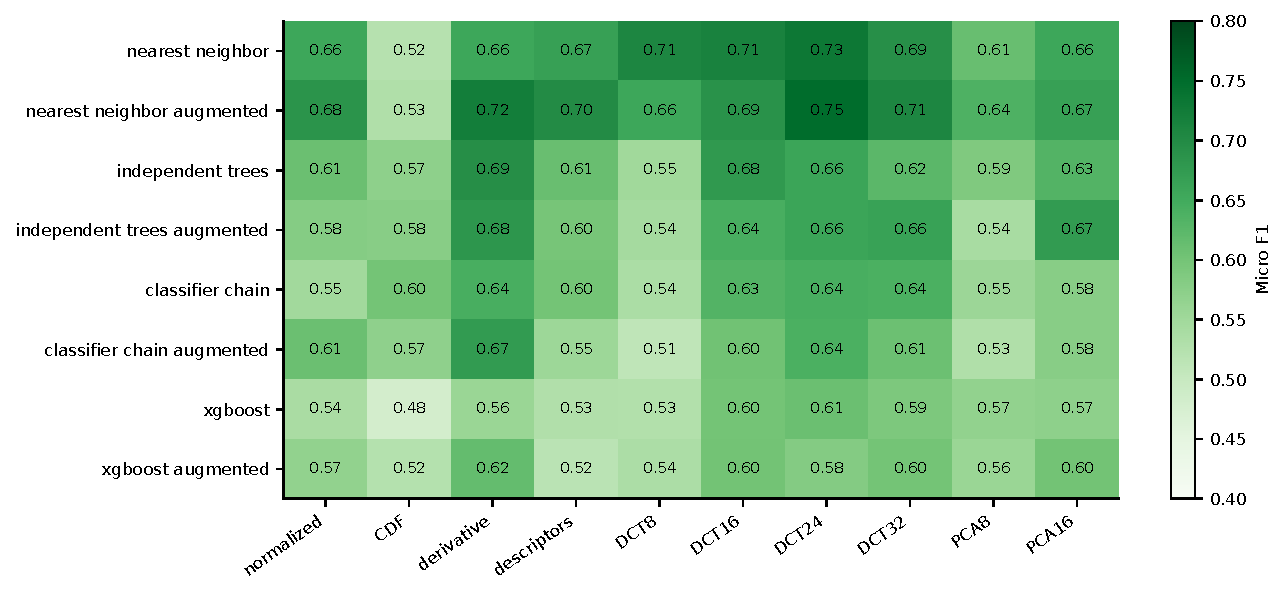
\includegraphics[width=\textwidth]{figures/SI_extensions_features.pdf}\caption{Fixed-feature nested ablations. Each cell uses training-only tuning, not outer-score feature selection.}\end{figure}

\clearpage\begin{figure}[p]\centering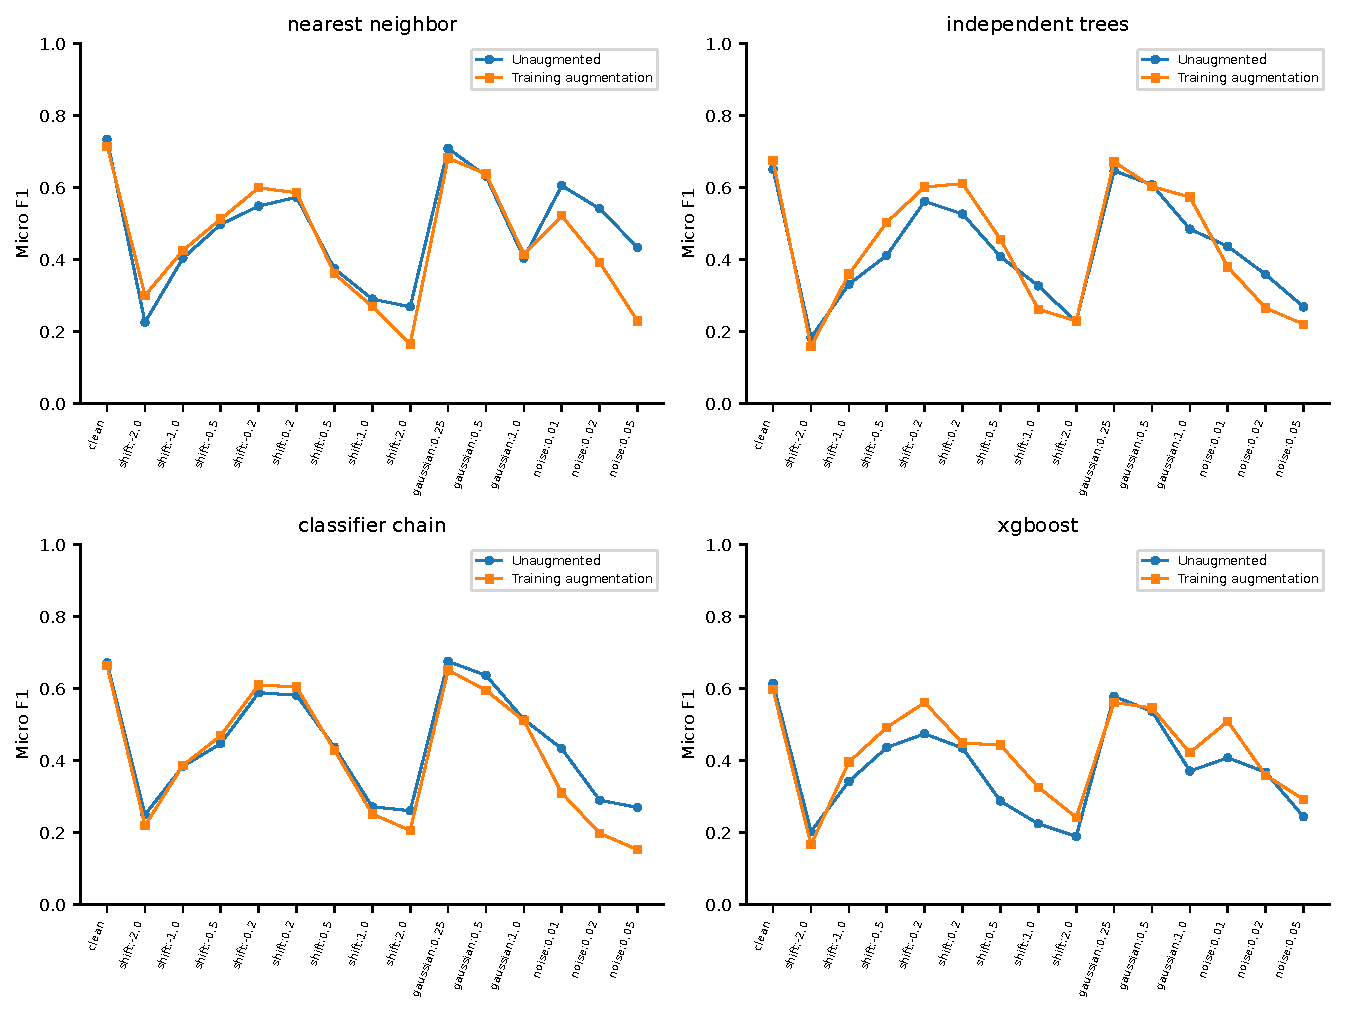
\includegraphics[width=\textwidth]{figures/SI_extensions_robustness.pdf}\caption{Clean and synthetic held-out stress scenarios for unaugmented and training-augmented recipes. These are not measured uncertainty distributions.}\end{figure}

\clearpage\begin{figure}[p]\centering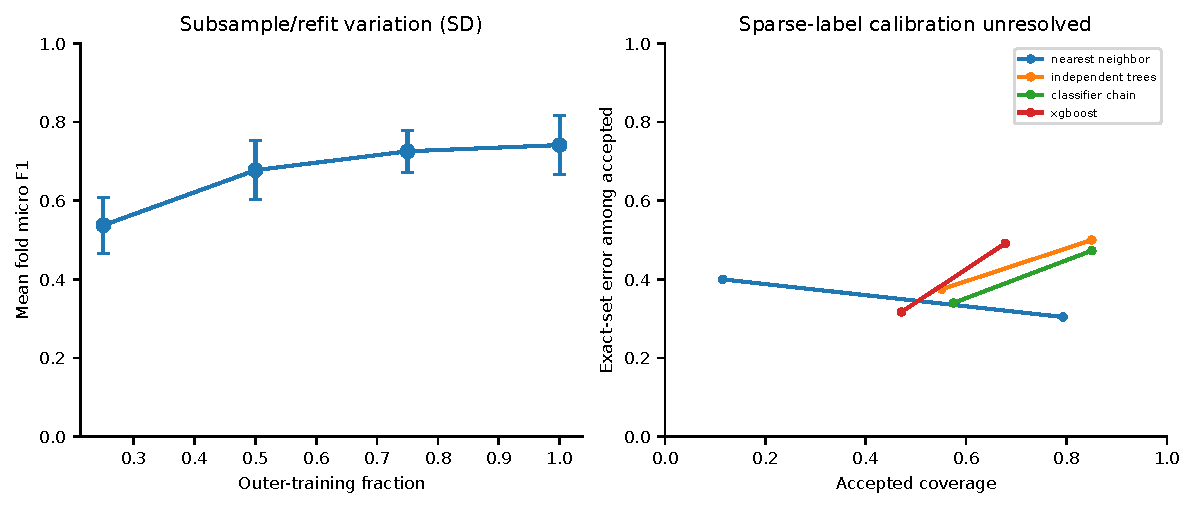
\includegraphics[width=\textwidth]{figures/SI_extensions_learning_review.pdf}\caption{Left: fold/subsample/refit mean and standard deviation, not a prospective confidence interval. Right: coverage versus exact-set error under the review rule; unsupported sparse labels prevent certified full-set calibration.}\end{figure}
